% import style file
\input audiotechnik.sty

% information about this document
\school{Bauhaus-Universität Weimar, Fakultät Medien, Lehrgebiet Audiotechnik SS 2011}
\supervisor{Dr.-Ing. Günther Schatter}
\supervisortwo{Dr. rer. nat. Dieter Kemter}
\title{Metadaten für Audio-/Radiosignale}
\subtitle{Übersicht zu Standards und zur Gewinnung}
\date{\today}
\author{
	\authorname{Malik Al-hallak}\\
	Bauhaus-Universität Weimar\\
	Fakultät Medien\\
	\authoremail{malik.al-hallak@uni-weimar.de}
\and
	\authorname{Julius Bullinger}\\
	Bauhaus-Universität Weimar\\
	Fakultät Medien\\
	\authoremail{julius.bullinger@uni-weimar.de}
}

% Abstrakt													1/2 Spalte
% Einleitung und kleine Scheißgrafik						3/2 Spalte
% Übersicht Standards, Vergleich, Schnittmengengrafiken
% EBUCore													1 Seite
% MPEG-7													1 Seite
% TV-Anytime												1 Seite
% Weitere													1/2 Seite
% Exkurs: Semantik Web, SKOS, RDF, OWL						1/2 bis 1 Seite
% Eigenleistung: 											2 Seiten
% Further Work, Future Ausblick								1/2 Seite

\begin{document}
	\maketitle
	
	\begin{abstract}
		\emph{In this paper, we describe the formatting guidelines
		for the workshop proceedings. Body text of the abstract
		should be 10 pt. Times New Roman Italic.}
	\end{abstract}
	
	\subsection{Keywords}
	Keywords are your choice, and are not mandatory.
	
	\section{Introduction}
	The proceedings are the records of the workshop. We hope to
	give these workshop byproducts a single, high-quality
	appearance. To do this, we ask that authors follow some simple
	guidelines. In essence, we ask you to make your paper look like
	this document. The easiest way to do this is simply to use this
	template and replace the content with your own material.
	
	\section{Page Size \& Page Limit}
	All material on each page should fit within a rectangle of 18x23.5
	cm, centered on the page, beginning 1.9 cm (.75") from the top of
	the page and ending with 2.54 cm (1") from the bottom. The right
	and left margins should be 1.9 cm. The text should be in two 8.45
	cm (3.33") columns with a .83 cm (.33") gutter. Camera-ready
	submissions should be about 8 pages in length or less.
	
	\section{Text \& Headings}
	For body text, please use a 10-point Times Roman font, or other
	Roman font with serifs, as close as possible in appearance to
	Times Roman in which these guidelines have been set. The goal is
	to have a 10-point text, as you see here. Please use sans-serif or 
	nonproportional fonts only for special purposes, such as
	distinguishing source code text. If Times New Roman is not available,
	try the font named Computer Modern Roman. On a Macintosh, use the
	font named Times. Right margins should be justified, not ragged.
	\par
	The following is an example of what a bulleted list should look like:
	\begin{itemize}
		\item All bullets should start at the same point.
		\item Spacing between the bullets can vary to produce
			  good column and page breaks.
		\item The use of hanging indent is recommended.
		\item Numbered lists should follow similar layout.
	\end{itemize}
	
	\subsection{Title and Authors}
	The title (Helvetica\footnote{If Helvetica is not available on your
	machine, Arial may be used as a substitute.} 16-point bold), authors’
	names (Helvetica 12-point-Bold) and affiliations (Times New Roman
	10-point) run across the full width of the page. We also recommend
	e-mail addresses for all authors. See the top of this page for three
	addresses. If only one address is needed, center all address text.
	For two addresses, use two centered columns, and so on. If more than
	three authors, you may have to improvise.\footnote{If necessary, you
	may place some address information in a footnote, or in a named section
	at the end of your paper. Please make footnotes Times New Roman 8 pt.}
	
	\subsection{Subsequent Pages}
	For pages other than the first page, start at the top of the page, and
	continue in double-column format. The two columns on the last page
	should be as close to equal length as possible.
	
	\begin{table}[htbp]\small
		\caption{Table captions should be placed above the table}
		\begin{tabularx}{\columnwidth}{ |c|c|>{\tblc}X|>{\tblc}X| }                    \hline
			Graphics & Top    & In-between & Bottom                                 \\ \hline
			Figures  & Good   & \multicolumn{2}{c|}{ Body text for the tables }     \\ \cline{1-2}
			Text     & Graphs & \multicolumn{2}{c|}{ should be Times Roman 10 pt. } \\ \hline
		\end{tabularx}
	\end{table}
	
	\subsection{References and Citations}
	Footnotes should be Times New Roman 8-point, and ragged right. Ragged
	right was decided because of many web addresses being used.
	\par
	A numbered list at the end of the article, ordered alphabetically by
	first author, and referenced by numbers in brackets \cite{Panther:2008}.
	See the examples of citations at the end of this document. Within this
	template file, use the style named references for the text of your
	citation. The body text of the citation/references section should be
	10 pt. Times New Roman.
	\par
	References should be published materials accessible to the public.
	Internal technical reports may be cited only if they are easily accessible 
	(i.e., give the address to obtain the report within your citation) and may
	be obtained by any reader. Private communications can be acknowledged, not
	referenced (e.g., "[Robertson, personal communication]"). Proprietary
	information may not be cited.
	
	\subsection{Page Numbering, Headers and Footers}
	Do not include headers, footers or page numbers in your submission.
	These will be added when the publications are assembled.
		
	% place this command somewhere in the first column of the last page
	% in order to balance the columns on the last page
	\balance
	
	\section{Figures/Captions}
	Place tables/figures/images in text as close to the reference as possible
	(see Figure~\ref{myfigure}). Figures may extend across both columns to a
	maximum width of 17.78 cm (7").
	\par
	Captions should be Helvetica bold 9-point. They should be numbered (e.g.,
	"Table 1" or "Figure 2"). Please note that the words "Table" and "Figure"
	are spelled out. Figure captions should be centered beneath the image or
	picture, and table captions should be centered above the table body.
	
	\begin{figure}[htbp]
		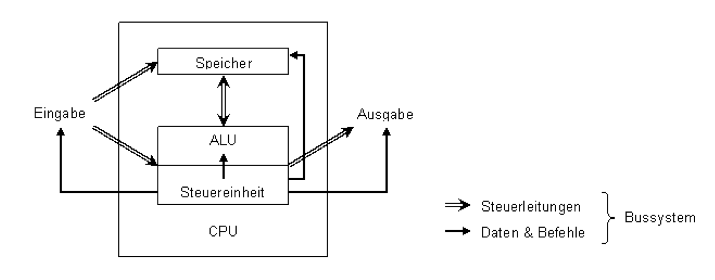
\includegraphics[width=\columnwidth]{images/beispiel.png}
		\caption{Place caption below the figure}
		\label{myfigure}
	\end{figure}
	
	\section{Equations}
	Equations look very pretty in \LaTeX. Here's a nifty example of a matrix:
	
	\begin{equation}
	 A_{mn} =
	 \begin{pmatrix}
	  a_{11} & a_{12} & \cdots & a_{1n} \\
	  a_{21} & a_{22} & \cdots & a_{2n} \\
	  \vdots  & \vdots  & \ddots & \vdots  \\
	  a_{m1} & a_{m2} & \cdots & a_{mn}
	 \end{pmatrix}
	\end{equation}
	
	Try that with MS Word! Now, let's have a look at the prettiness 
	of Equations~\ref{myequation} and~\ref{myequation2}:
	
	\begin{equation}
		f(n) = \left\{ 
			\begin{array}{l l}
			n/2 & \quad \text{if $n$ is even}\\
			-(n+1)/2 & \quad \text{if $n$ is odd}\\
		\end{array} \right.
		\label{myequation}
	\end{equation}
	
	\begin{equation}
		\int_{- \frac{\pi}{2}}^{\frac{\pi}{2}}cos(\omega t)~dt
		~=~
		\frac{2}{\omega}sin( \frac{1}{2}\omega \pi)
		\label{myequation2}
	\end{equation}
	
	\section{Section Heads}
	The heading of a section should be in Helvetica Bold 10-point bold, in
	all-capitals flush left with an additional 6 points of white space above
	the section head. Sections and subsequent subsections should flush left.
	
	\subsection{Subsections}
	The heading of subsections should be in Helvetica 10-point bold with
	only the initial letters capitalized. For subsections and subsubsections,
	a word like \emph{the} or \emph{a} is not capitalized unless it is the
	first word of the header.
	
	\subsubsection{Subsubsections}
	The heading for subsubsections should be in Helvetica 10-point italic
	with initial letters capitalized and 6 points of white space above the
	subsubsection head.
	
	\section{Acknowledgements}
	Your appreciation to employers, co-workers, department heads, and/or
	institutions that issued you a grant can be acknowledged in this section.
	\newpage
	
	\section {Der Metadaten Standard MPEG-7} 
	
	\subsection {\\Einleitung}
	
	Der MPEG-7 Standard wurde 2002 von der \emph{Moving Picture Expert Group} als ISO/IEC 15938 verabschiedet. Im Gegensatz zu den früheren MPEG Standards (MPEG-1, MPEG-2 und MPEG-4) kein Kompressionsstandard für multimediale Daten sondern ein Metadaten Standard für selbige.\\Er bietet eine auf XML-Basierende umfangreiche Repräsentation von Metainformation für Audio- und Videodaten.\\Im folgenden wird der Standard im hinblick auf Audiosignale detailliert vorgestellt und seine automatisch generierbaren Aspekte vorgestellt.
	
	\subsection{Inhalt}
	
	Der MPEG-7 Standard spezifiziert vier Bestandteile:
	
	\begin{itemize}
		\item \emph{Descriptors}
		\item \emph{Descriptor Schemes}
		\item \emph{Description Definition Language}
		\item \emph{Binary Format für MPEG-7}
	\end{itemize}
	
	\subsubsection {Descriptors (D)}
	
Der erste Teil des Standards sind \emph{Descriptors}. Diese arbeiten auf räumlichen, zeitlichen oder physischen Segmenten der Ressource und  halten Daten zur Repräsentation eines Merkmals der Audiodatei.\\Dabei werden entweder gleiche Zeitintervalle der Ressource beschrieben oder sie wird in Segmente unterteilt und und Ähnlichkeiten und Differenzen werden aufgezeichnet. Beispiele für solche Descriptors sind der \emph{AudioWaveform} Descriptor welcher einem Intervall des Signals z.B. maximaler und minimaler Tonfrequenz zuweist.\\ Diese Strukturen sind Low-Level und beinhalten lediglich die technischen Eigenschaften der Audio-Ressource. Es werden derzeit 17 \emph{Feature Descriptors} und ein spezieller \emph{Silence Descriptor} standardisiert. Diese 18 Strukturen sind in Untergruppen Organisiert (siehe Abb. 2).\\


\begin{figure}[h]
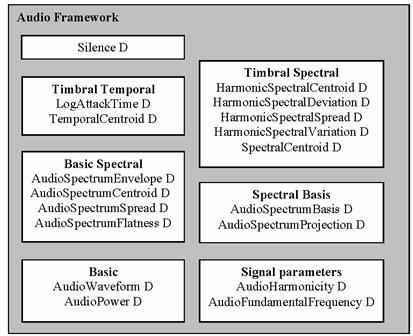
\includegraphics [scale=0.65]{image061.jpg}
\caption {Low-Level Descriptors in MPEG-7}
\end{figure}

Der \emph{Silence Descriptor} ist einfach die Darstellung das an dieser Stelle kein signifikanter Ton vorhanden ist und kann z.B. dazu eingesetzt werden ein Segment mit dieser Eigenschaft nicht weiter zu bearbeiten was die Erstellung der Metadaten effizienter macht.\\

	\subsubsection{Description Schemes (DS)}
		Der MPEG-7 Standard liefert neben den Low-Level Descriptors auch High-Level Description Tools in Form von \emph{Description Schemes}. Description Schemes beschreiben die Audiodatei auf einer höheren Abstraktionsebene und setzen dafür Descriptors und andere Description Schemes in Beziehung zueinander. \\Desciption Schemes nutzen die Rohdaten aus Descriptors und anderen Description Schemes um Audiodaten auf einem hohen Abstraktionsgrad zu beschreiben. Sodass Description Schemes die Struktur und die Semantik liefern in welcher die Descriptors und andere Description Schemes in Verbindung gesetzt wird. Damit kann man neben der rein technischen Low-Level Beschreibung der Ressource auch Charakteristiken wie Ton- , Instrumenten- und Melodie-Erkennung erzeugen und vermerken. \\
		
	\subsubsection{Description Definition Language (DDL)}
Neben den bereits genannten Möglichkeiten bietet der MPEG-7 Standard ein weiteres mächtiges Werkzeug. Mit der Description Definition Language ist es möglich weitere, auf die Anforderungen des jeweiligen Nutzers zugeschnittene, Descriptors und Description Schemes zu entwickeln.\\ Die Description Definition Language ist eine Erweiterung von XML-Schema.

\subsubsection{Binary Format für MPEG-7 BiM}

Das BiM ist entwickelt worden um die Metadaten schnell übertragen und streamen zu können. Das BiM bietet eine hohe Kompressionsrate der XML-Metadaten ( bis zu 98\%) und einen schnellen Zugriff auf Daten Entitäten im komprimierten Stream
\begin{figure}[h]
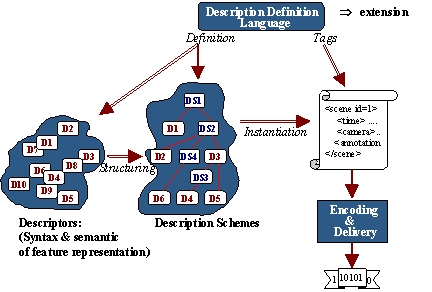
\includegraphics [scale=0.55]{image004.jpg}
\caption {MPEG-7 Aufbau}
\end{figure}


	\newpage
	\section{DER METADATEN STANDARD EBUCore}
	
	\subsection{\\Einleitung\\}
	Der EBUCore ist ein Metadatenset welches von der \emph{European Broadcasting Union (EBU)} entwickelt wurde. Die EBU ist ein Zusammenschluss von 74 Rundfunkanstalten  in 56 Ländern Europas, Nordafrikas und Vorderasiens. Dieser Zusammenschluss produziert z.B. auch den Eurovision Song Contest.\\ Der EBUCore ist eine Erweiterung des \emph{DublinCore}, welcher 1995 in Dublin/Ohio festgesetzt wurde. Der DublinCore spezifiziert eine Reihe von Metadaten zur beschreibung von Dokumenten im Internet.\\ Im Jahr 2000 war es das anfängliche Ziel der EBU den DublinCore auf Audioarchive zu übertragen. Dieses Ziel wurde 2008 erweitert. Das neue Ziel war es den EBUCore so zu erweitern, das man mit den Metadaten nicht nur Daten im Archiv beschreiben kann, sondern mit ihrer Hilfe auch Archive durch z.B. Suchmaschinen im Browser durchsuchen kann.\\Die EBU sagt, dass heutige Ziele nicht mehr auf Audioressourcen und Archive beschränkt ist.\\Der bekanntesten Einsatzort des EBUCore ist derzeit die \emph{Europeana}. Die Europeana ist ein Projekt welches darauf abzielt, das kulturelle Erbe Europas zu digitalisieren und für jedermann zugänglich zu machen. Mithilfe des Webportals hat man Zugriff auf viele Millionen multimediale Ressourcen aus Europa und der Welt.\\Damit man diese Ressourcen auch nach der gewünschten durchsuchen kann, braucht es ein einheitliches Metadaten Format für Europa.
	
	\subsection{\\Der Standard\\}
	Der EBUCore ist eine minimale Liste von Attributen die man benötigt um eine multimediale Ressource zu beschreiben.Getreu dem Motto :\begin{quote}Wenn du's nicht findest, hast du's auch nicht.\end{quote} versucht die EBU durch den EBUCore einen allumfassenden Standard bereit zu stellen welcher eine Verbindung zwischen kulturellen Datenbanken, Produzenten multimedialer Ressourcen, Rundfunkanstalten, Archiven und Netzontologien herstellt.\\
Auch der EBUCore nutzt das XML Format zur Repräsentation der Metainformation. Der Standard ist unter anderem in der EBU tech3293 spezifiziert.\\Anders als der MPEG-7 Standard muss der EBUCore komplett manuell erstellt werden. Dazu wird einfach ein XML-Instanz Dokument erstellt welches dem XML-Schema entsprechen muss.\\Das XML-Schema definiert über 30 Tags welche zur Beschreibung der Ressource dienen. Dabei werden neben den üblichen Beschreibungsformen, wie Titel oder Sprache, auch Tags angeboten die Informationen über das physikalische oder digitale  Format, Version oder Herausgabe Historie. Diese Tags spiegeln hier beispielhaft das bestreben produzierenden und konsumierende Gruppen unter einen Standard zusammen zu fassen.\\
Es folgen nun zwei Beispiele wie ein XML-Instanz Dokument für ein Bild und eine Audioressource aussehen kann. Dabei kann man gut erkennen das der Standard komplett unabhängig von der zu beschreibenden Ressource fungiert.

\begin{lstlisting}[caption=Beispiel-XML EBUCore für Albrecht Dürers Bild: Adam und Eva]{Name}

<?xml version="1.0" encoding="UTF-8"?>
<schema xmlns:xsi=
"http://www.w3.org/2001/XMLSchema-instance" ...>

  <ebuCoreMain>
    <coreMetadataType>
      <title>Adam and Eve</title>
      <creator>Duerer, Albrecht (german painter, 1471-1528) </creator>
      <description>...</description>
      <source>VADS</source>  
      <rights>Rights Owner: The Bowes Museum Castle, Co. Durham</rights>
      <provider>CultureGrid; UK</provider>
      <subject>religion (Adam and Eve)</subject>
      <type>Physical Object</type>
    </coreMetadataType>
  </ebuCoreMain>
</schema>
\end{lstlisting}


\begin{lstlisting}[caption=Beispiel-XML EBUCore für die Europahymne]{Name}

<?xml version="1.0" encoding="UTF-8"?>
<schema xmlns:xsi=
"http://www.w3.org/2001/XMLSchema-instance" ...>

  <ebuCoreMain>
    <coreMetadataType>
      <title>Europahymne ; Hymne europeen ; European anthem</title>
      <creator>van Beethoven, Ludwig</creator>
      <description>...</description>
      <source>Dernier mouvement de la Neuvieme symphonie (Ode a la joie) / van Beethoven, Ludwig (compositeur); ...</source>  
      <rights>Centre Virtuel de la Connaissance sur l Europe (CVCE)</rights>
      <provider>ASSETS; Luxembourg</provider>
      <language>fr; en; de</language>
      <identifier>doi_cvce_audiovisual_4b6e5671-a0fc-45fa-8368-f84e4817dc14></identifier>
      <type>Physical Object</type>
    </coreMetadataType>
  </ebuCoreMain>
</schema>
\end{lstlisting}


	\newpage
	
	\section{Verhältnis zwischen XML und RDF/OWL (Semantic Web) und SKOS für classification schemes}
	Absatz

	\subsection{RDF, RDFS und RDF/XML}
	\subsubsection{RDF}
	Das Resource Description Framework (RDF) ist eine universelle formale Sprache zur Beschreibung von strukturierten Informationen (ursprünglich: Metadaten im Web). Mittels RDF werden Information über so genannte Ressourcen gespeichert. Ressourcen sind Uniform Ressource Identifiers (URIs), die eine Quelle referenzieren. Diese Ressourcen können Webseiten, ISBNs für Bücher und Zeitschriften oder DOIs (zum Beispiel doi:10.1000/182) sein.
	
	Metadaten werden als Tripel -- Subjekt, Prädikat, Objekt -- gespeichert. Dabei wird die Beziehung zwischen Subjekt und Objekt angegeben. Die Beziehung \enquote{\enquote{Die Glocke} ist von Friedrich Schiller geschrieben} ergibt das Tripel \enquote{Die Glocke} (Subjekt), \enquote{ist geschrieben von} (Prädikat), \enquote{Friedrich Schiller} (Objekt). Zur Notation nutzt man häufig die (inoffizielle) \emph{Turtle}-Syntax. % Obiges Trippel sieht in dann so aus: % TODO: evtl. Turtle-Syntax
	Auf diese soll hier jedoch nicht eingegangen werden, da in der Praxis überwiegend die Serialisierung mittels Extensible Markup Language (XML) genutzt wird.
	
	\subsubsection{RDF/XML}
	Dieses vom W3C standardisierte Format wird RDF/XML gennant. \prettyref{lis:rdfxml} zeigt ein Beispiel für obige Beziehung in RDF/XML. Dabei wurden zusätzlich einige Elemente der Dublin-Core-Spezifikation genutzt.
	% TODO: placement on the same page!
	\lstinputlisting[float=*b, language=XML, caption=Beispiel für XML/RDF, label=lis:rdfxml]{files/schiller.rdf}

	\subsubsection{RDFS}
	RDF benötigen zur \emph{Interpretation} der dargestellten Beziehungen ein gemeinsames Vokabular, zum Beispiel Dublin Core. RDF Schema (RDFS) stellen dafür ein Vokabular zur Verfügung, mit dessen Hilfe innerhalb von RDFS-Dokumenten Aussagen über semantische Beziehungen der Termini gemacht werden können. Es handelt sich dabei nicht um ein thematisches Vokabular; vielmehr 

	\subsection{OWL}
	Web Ontology Language (OWL) ist eine Spezifikation des W3C, die entwickelt wurde, um...
	
	OWL basiert auf RDF/XML, fügt jedoch weitere Ausdrücke zur Beschreibung von Eigenschaften und Klassen hinzu. Damit werden Aussagen ähnlich der Prädikatenlogik ermöglicht (Disjunktheit, Aussage "genau einer", Äquivalenz...)
	
	OWL bietet drei Untersprachen mit steigender Ausdrucksstärke (\emph{OWL Lite}, \emph{DL} (description logic) und \emph{Full}) und unterschiedlichen Zielgruppen. OWL Lite ist eine (echte) Teilsprache von OWL DL, welches wiederrum eine (echte) Teilsprache von OWL Full ist.
	
	% http://www.semaweb.org/dokumente/w3/TR/2004/REC-owl-features-20040210-DE.html, 28.05.2011, 13:13
	% Hitzler, Pascal, et. al. Semantic Web,	Berlin [u.a.] Springer, 2008, Seite 127
	
	\subsubsection{OWL 2}
	% TODO
	
	\subsection{SKOS}
	Simple Knowledge Organization System (SKOS) ist eine vom W3C spezifierte formale Sprache zum Verteilen und Verlinken von Informationsystemen wie Thesauri, Taxonomien und Normdateien im Web. SKOS basiert auf RDF und RDFS.
	% http://www.w3.org/TR/skos-reference/, 28.05.2011, 15:27
	
	...
	
	SKOS soll die Nutzung von concept schemes im Web im Vergleich zu OWL erleichtern. OWL verfolgt das Ziel, komplexe Konzeptstrukturen auszudrücken, um so ausführliche Metadaten zu generieren und Schlussfolgerungswerkzeuge zu unterstützen. Die Erstellung sinnvoller Web-Ontologien ist jedoch sehr aufwändig, und in vielen Fällen werden die zahlreichen Möglichkeiten der OWL nicht benötigt. Deshalb kann hier der Einsatz von SKOS vorteilhaft sein.
	
	% http://en.wikipedia.org/wiki/Simple_Knowledge_Organization_System vom 13:30, 12 May 2011. 28. Mai 2011, 15:37
	
	\bibliographystyle{phcpc}
	\bibliography{references}
\end{document}